\documentclass[11pt,a4paper,spanish]{book}  % book, article

\usepackage[english]{babel}
\usepackage[utf8]{inputenc}
% Paquetes para incluir graficos:
\usepackage{graphics}
\usepackage{graphicx}
\usepackage{epstopdf}
% Tratamiento de graficos
\usepackage{picture}
% Colores
\usepackage[usenames]{color}
% Texto preformateado
\usepackage{verbatim}
\usepackage{listings}
% Hipervinculos (indice y URLs)
\usepackage{hyperref}
% Matematicas
\usepackage{amsfonts}
\usepackage{amsmath}
\usepackage{amsthm}
\usepackage{amssymb}
\usepackage{anysize}
\usepackage{caption}
\usepackage{geometry}
\usepackage[final]{pdfpages}
\usepackage{cite}
\usepackage{natbib}
\usepackage[numbib,notlof,notlot,nottoc]{tocbibind}

\newcommand{\HRule}{\rule{\linewidth}{0.5mm}}

%%PER EL CODI EN C%%%
\usepackage{listings}
\lstset{ %
language=C++,                % choose the language of the code
basicstyle=\footnotesize,       % the size of the fonts that are used for the code
numbers=left,                   % where to put the line-numbers
numberstyle=\footnotesize,      % the size of the fonts that are used for the line-numbers
stepnumber=1,                   % the step between two line-numbers. If it is 1 each line will be numbered
numbersep=5pt,                  % how far the line-numbers are from the code
backgroundcolor=\color{white},  % choose the background color. You must add \usepackage{color}
showspaces=false,               % show spaces adding particular underscores
showstringspaces=false,         % underline spaces within strings
showtabs=false,                 % show tabs within strings adding particular underscores
frame=single,           % adds a frame around the code
tabsize=2,          % sets default tabsize to 2 spaces
captionpos=b,           % sets the caption-position to bottom
breaklines=true,        % sets automatic line breaking
breakatwhitespace=false,    % sets if automatic breaks should only happen at whitespace
escapeinside={\%*}{*)}          % if you want to add a comment within your code
}

%%%%%%%% Entornos teorema, definiciÛn, comentario, ... %%%%%%%%
\swapnumbers  % Poner el numero del teorema ANTES del teorema.

\theoremstyle{definition}  % Titulo en negrita y texto plano

\newtheorem{definicion}{Definicion}[chapter]
\newtheorem{ejemplo}[definicion]{Ejemplo}
\newtheorem{comentario}[definicion]{Comentario}
\newtheorem{propiedades}[definicion]{Propiedades}
\newtheorem*{objetivo}{Objetivo}
\newtheorem*{idea}{Idea}

\theoremstyle{plain}  % Titulo en negrita y texto en cursiva.
\newtheorem{teorema}[definicion]{Teorema}
\newtheorem{proposicion}[definicion]{ProposiciÛn}
\newtheorem{corolario}[definicion]{Corolario}
\newtheorem{lema}[definicion]{Lema}

\theoremstyle{remark}  % Titulo en cursiva y texto plano
\newtheorem*{observacion}{ObservaciÛn}
\newtheorem*{ejercicio}{Ejercicio propuesto}
\newtheorem*{pregunta}{Pregunta}

%%%%%%%% Formato cÛdigo incluido %%%%%%%% 
\lstset{ %
%language=Octave,                % choose the language of the code
basicstyle=\footnotesize,       % the size of the fonts that are used for the code
numbers=left,                   % where to put the line-numbers
numberstyle=\footnotesize,      % the size of the fonts that are used for the line-numbers
stepnumber=1,                   % the step between two line-numbers. If it's 1 each line 
                                % will be numbered
numbersep=5pt,                  % how far the line-numbers are from the code
%backgroundcolor=\color[rgb]{0.8,0.8,0.8},  % choose the background color. You must add \usepackage{color}
showspaces=false,               % show spaces adding particular underscores
showstringspaces=false,         % underline spaces within strings
showtabs=false,                 % show tabs within strings adding particular underscores
frame=single,	                % adds a frame around the code
tabsize=2,	                % sets default tabsize to 2 spaces
captionpos=b,                   % sets the caption-position to bottom
breaklines=true,                % sets automatic line breaking
breakatwhitespace=false,        % sets if automatic breaks should only happen at whitespace
title=\lstname,                 % show the filename of files included with \lstinputlisting;
                                % also try caption instead of title
escapeinside={\%*}{*)},         % if you want to add a comment within your code
morekeywords={*,...}            % if you want to add more keywords to the set
}




%\marginsize{3 cm}{2 cm}{2 cm}{2.5 cm}

%\title{\textbf{Project Handbook for Development Projects}}
%\author{Carolina Millet \\ Xavier Bush}
%\date{October 2014}		% Comentar para que aparezca la fecha de hoy
\newgeometry{
    top=35mm,
    bottom=30mm,
    outer=30mm,
    inner=30mm,
}

\begin{document}


\begin{titlepage}
\begin{center}


\textsc{\LARGE Kungliga Tekniska Högskolan}\\[1.5cm]

\textsc{\Large ~}\\[-0.5cm]


{ \huge \bfseries \textbf{Project Report} \\

\HRule

 Noise and echo cancellation in a teleconference\\[0.4cm]}

\HRule \\[1.1cm]

		\begin{figure}[h]
		\centering
		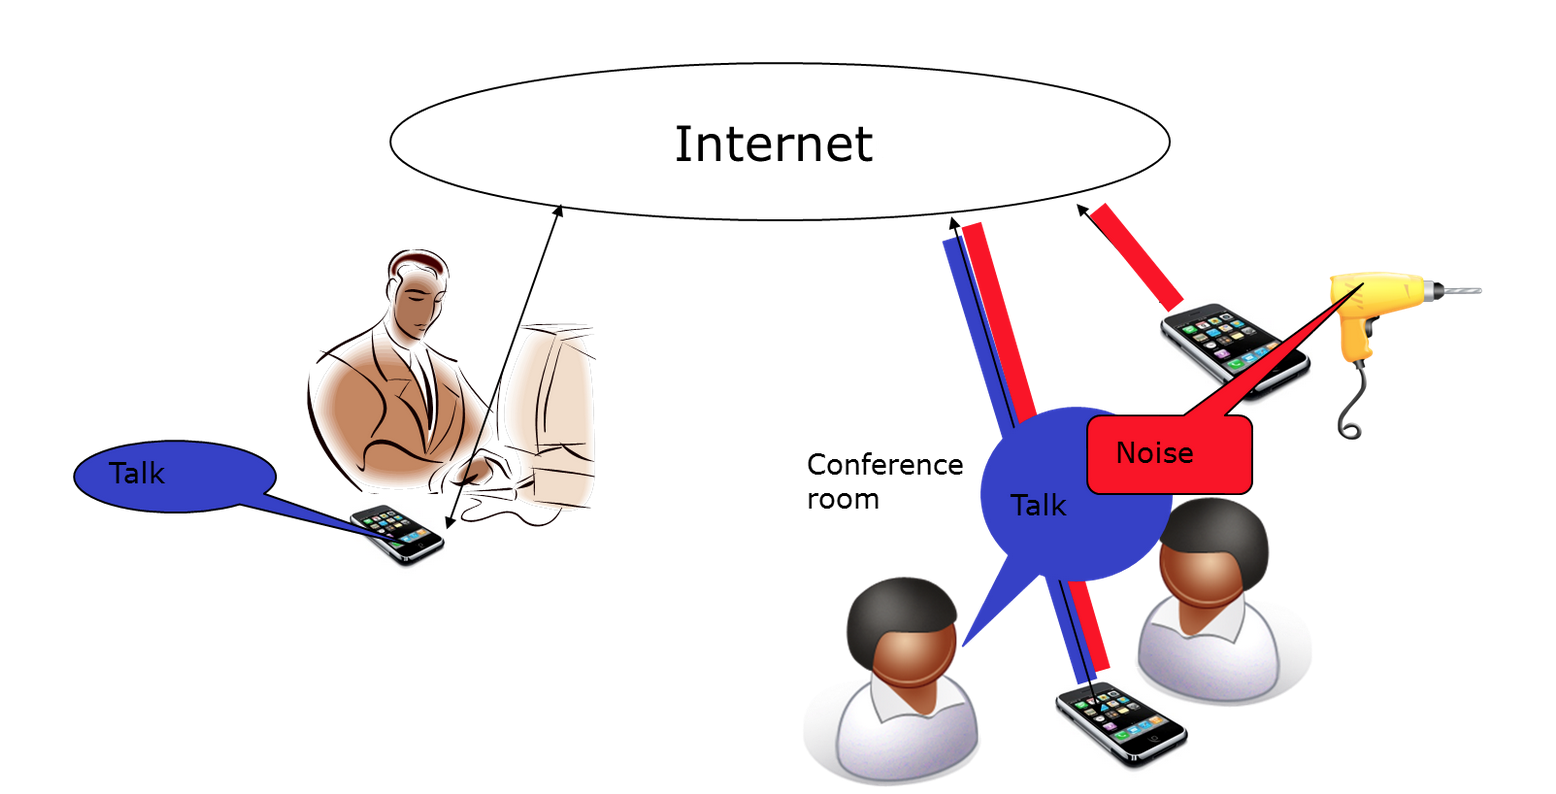
\includegraphics[width=10cm]{images/other/scenario}
		\label{scenario}
		\end{figure}

% Author and supervisor
\begin{minipage}{0.4\textwidth}
\begin{flushleft}
\emph{Authors:}\\
Animesh DAS \\ Jonas SEDIN \\ Mohammad ABDULLA \\ Thomas GAUDY \\ Xavier BUSH
\end{flushleft}
\end{minipage}
~
\begin{minipage}{0.4\textwidth}
\begin{flushright}
\emph{Advisor:}\\
Per ZETTERBERG
\end{flushright}
\end{minipage}

\vfill

% Bottom of the page
{\large Spring 2015} \\[1cm]
\end{center}



\end{titlepage}
\restoregeometry



\pagebreak\tableofcontents
\pagebreak

\chapter{Background}

	\section{Introduction of noisy environments}
	\label{sec:intronoise}
	
It is a fact that the scenarios with phone calls involved are increasing every day. This situation implies an increase of the probability of being in a noisy scenario, specially in big cities. As a result of the discomfort that the users suffer in these noisy environments, engineering and science have worked with different approaches to solve this problem.

The diversity of noise nature and its sources lead the engineering to a big challenge: develop high performance soltions in these diverse environments. When facing noise cancellation is very important to take into account the variability that the noise may experience, as previously said. Duration of the noise sequences (from \textit{ms} to long sequences), color of the noise and stationarity are possible classifications of the noise and each classification implies different ways of treating it. Therefore, a lot of systems are using combined techniques to reach the best possible performance, which has been naturally the case of this project.

	\section{Historical Overview}
	Before presenting the proposed solutions and approaches of the project, it is needed a historical overview to understand how have the group been influenced and which have been the patterns of research.


	\section{Description of the project}
	\label{sec:introproblem}
	
	The problem proposed by the course \textit{EQ2440} has been a "Noise and echo cancellation of a teleconference". The general scenario is that the first of the two speakers of the teleconference is in a noisy environment and the clear goal is to cancel as much noise as possible in order that the second speaker could receive a cleaner speech and make the conversation more comfortable. As said in \ref{sec_intronoise}, there are different approaches to solve this problem, where several of them require the availability of pure noise recordings, in our case recorded with a third phone placed close to the noise source. To have a clearer overview of the scenario the Figure \ref{scenario2} shows an approximate scheme easy to understand.
	
	When talking about denoising a teleconference there are two factors to take into account, techniques to cancel the noise and the possibility of their implementation in a real time application. The real time application has been, as expected, a big challenge because it implies good performance in terms of cancellation with the minimum reachable delay to conserve the naturalness of the conversation.
	
		\begin{figure}[h]
		\centering
		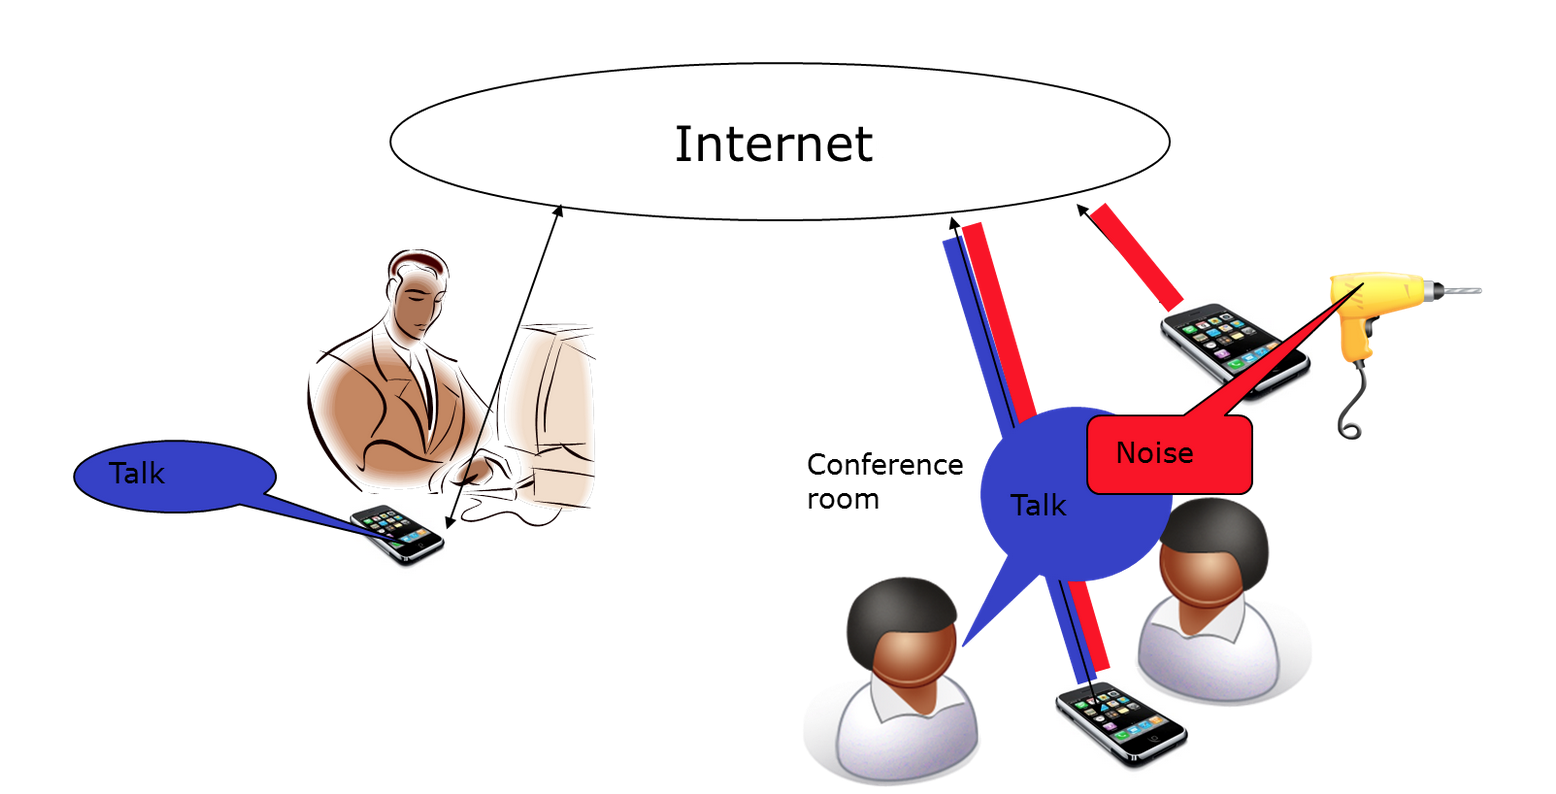
\includegraphics[width=10cm]{images/other/scenario}
		\caption{Scenario to solve}
		\label{scenario2}
		\end{figure}
	
	
	
	\section{Goal}
	As commented in \ref{sec:introproblem}, the goal is to cancel the noise contribution in the conversation between the two speakers of the teleconferences. With the purpose to simplify the scenario, it will be assumed that only one of the speakers is surrounded by noise and the main noise source is known as well.
	
	As in every engineering project, the group had to find a compromise between performance in noise cancellation and viability of implementation in real life. As it will be explained in \ref{sec:methodology}, the computational cost is a big constrain and the best performance of certain approaches (\ref{sec:theory}) introduce too much delay because of this reason. As a consequence, not always the best solution will be possible to implement in the real time version of the project.
	
	As a contrast, the personal goals of the project members are to learn form the teamwork environment, learn a research methodology, research criteria and certain skills of management that might be used in the performance of a Master Thesis (as an inmidate future) and in a research or business environment.
	
	The new knowledge acquisition is obviously another personal goal of all the team members.
	
	
	
	
	\section{Organizationn and Human Resources}

The organization of the project consists in electrical engineering students at different stages of the studies and within different specializations. In order to make the team as efficient as possible, the project has been divided in four different groups: \textit{Theory Group}, \textit{Android Group}, \textit{Multimedia Group} and \textit{Management Group}, all of them explained in detail in \ref{sec:methodology}.

In terms of making easier the transfer of information between groups, the makeup of the groups has followed a cross-specialization criteria. Therefore, there are team members in more than one group, and it has been possible due to the wide scope of skills that the team members have.

The distribution of the team members has been as follows.

\begin{itemize}

\item Animesh Das
	\begin{itemize}
	\item Role: Management Group
	\item e-mail:animeshu1989@gmail.com (animeshd@kth.se)
	\item Telephone: +46 737155575
	\end{itemize}
	
\item Jonas Sedin
	\begin{itemize}
	\item Role: Theory Group \& Android Group
	\item e-mail: sedinjo@gmail.com (jonassed@kth.se)
	\item Telephone: +46 704252951
	\end{itemize}
	
\item Mohammad Abdulla
	\begin{itemize}
	\item Role: Android Group \& Multimedia Group
	\item e-mail: hamodiilatch@gmail.com (mabdulla@kth.se)
	\item Telephone: +46 737393276
	\end{itemize}
	
\item Thomas Gaudy
	\begin{itemize}
	\item Role: Android Group
	\item e-mail: gaudy.thomas@gmail.com (gaudy@kth.se)
	\item Telephone: +46 760936034
	\end{itemize}
	
\item Xavier Bush
	\begin{itemize}
	\item Role: Theory Group \& Management Group (Project Leader)
	\item e-mail: xavier.bush@gmail.com (xbush@kth.se)
	\item Telephone: +46 764141834
	\end{itemize}
	
	
\end{itemize}

The sponsor members as Project Examiner/Supervisor and Project Support are:

\begin{itemize}
\item Per Zetterberg
	\begin{itemize}
	\item Role: Project Examiner
	\item e-mail: perz@ee.kth.se
	\item Telephone: +46 8 790 77 85
	\end{itemize}
	
\item Hadi Ghauch
	\begin{itemize}
	\item Role: Group Assistant
	\item e-mail: ghauch@kth.se
	\end{itemize}
	
\item Martin Ohlsson
	\begin{itemize}
	\item Role: Android Guru
	\item e-mail: martinoh@kth.se
	\item Telephone: +46 87907818
	\end{itemize}
\end{itemize}

\chapter{Methodology}
\label{sec:methodology}

This chapter shows the methodology that the group has followed since the projecte started. On the first hand, it goes without saying that the project group has followed the \textit{Scientific Method} in the implementation of the project. On the second hand, the 


\begin{itemize}
\item \textit{Theory Group}: its goal is to find theory solutions for the noise cancellation problem having in mind potential computational problems.
\item \textit{Android Group}: its goal is to implement in Android the solutions given by the \textit{Theory Group}. This group will handle as well all the technical aspects of the communication between the mobilephones.
\item \textit{Multimedia Group}: the purpose of the group is to create the presentations and video to show the results of the project
\item \textit{Management Group}: the drawing up of the Project Plan, Progress Report and Project Report are the main duties of this group, as well as the creation of all the tools needed to make a good follow up of the work in the project. 
\end{itemize}



\section{Management Group}

\section{Theory Group}

\section{Android Group}

\section{Multimedia Group}

\section{Cross-Duties}


\chapter{Theory}
\label{sec:theory}

\chapter{Android}

\chapter{Conclusions}

%\include{Chapter1}			% Incluye "Chapter1.tex"


%%%%%%%% Fin del documento %%%%%%%% 
\end{document}